\section{Results}
\label{results}
This section quantifies
the effects of~\acdc{} and determines if the performance of DCTCP
implemented in the vSwitch (\ie{}, \acdc{}) is equivalent to
the performance of DCTCP implemented in the host TCP stack.

\tightparagraph{Testbed}
The experiments are conducted on a physical testbed with 17 
IBM System x3620 M3 servers (6-core Intel Xeon
2.53GHz CPUs, 60GB memory) and Mellanox ConnectX-2 EN 10GbE NICs.
Our switches are IBM G8264, each with a buffer of 9MB shared
by forty-eight 10G ports. 
%The switches have dynamic memory management enabled by default.

\tightparagraph{System settings}
We run Linux kernel 3.18.0 which implements DCTCP as a 
pluggable module.
We set {{\tt $RTO_{min}$} to 10 ms~\cite{vasudevan2009safe,judd2015nsdi} and
set {\tt tcp\_no\_metrics\_save}, {\tt tcp\_sack} and {\tt tcp\_low\_latency} to 1.
\crs{Results are obtained with MTU sizes of 1.5KB and 9KB,
as networks typically use one of these settings. 
Due to space constraints, a subset of
the results are presented and unless otherwise noted, the MTU is set to 9KB.}



\tightparagraph{Experiment details}
To understand~\acdc{} performance, three different congestion control configurations
are considered. The baseline scheme, referred to as {\em CUBIC}, configures
the host TCP stack as CUBIC (Linux's default congestion control), which runs on top of an unmodified version of OVS.
Our goal is to be similar to {\em DCTCP}, which configures the host TCP
stack as DCTCP and runs on top of an unmodified version of OVS. Our scheme,{\em ~\acdc{}},
configures the host TCP stack as CUBIC (unless otherwise stated) and implements DCTCP congestion control in OVS.
In DCTCP and~\acdc{}, WRED/ECN is configured on the switches. In CUBIC,
WRED/ECN is not configured.

The metrics used are: TCP RTT (measured by sockperf~\cite{sockperf}),
TCP throughput (measured by iperf),
loss rate (by collecting switch counters) and
Jain's fairness index~\cite{jain-index}.
In \cref{macro}, flow completion time (FCT)~\cite{dukkipati2006flow} is used 
to quantify application performance.~\crs{All benchmark tools are run
in a container on each server, rather than in a VM.}

\subsection{Microbenchmarks}
\label{micro}
\begin{figure}[!t]
        \centering
        \begin{subfigure}[b]{0.45\textwidth}
                \centering
                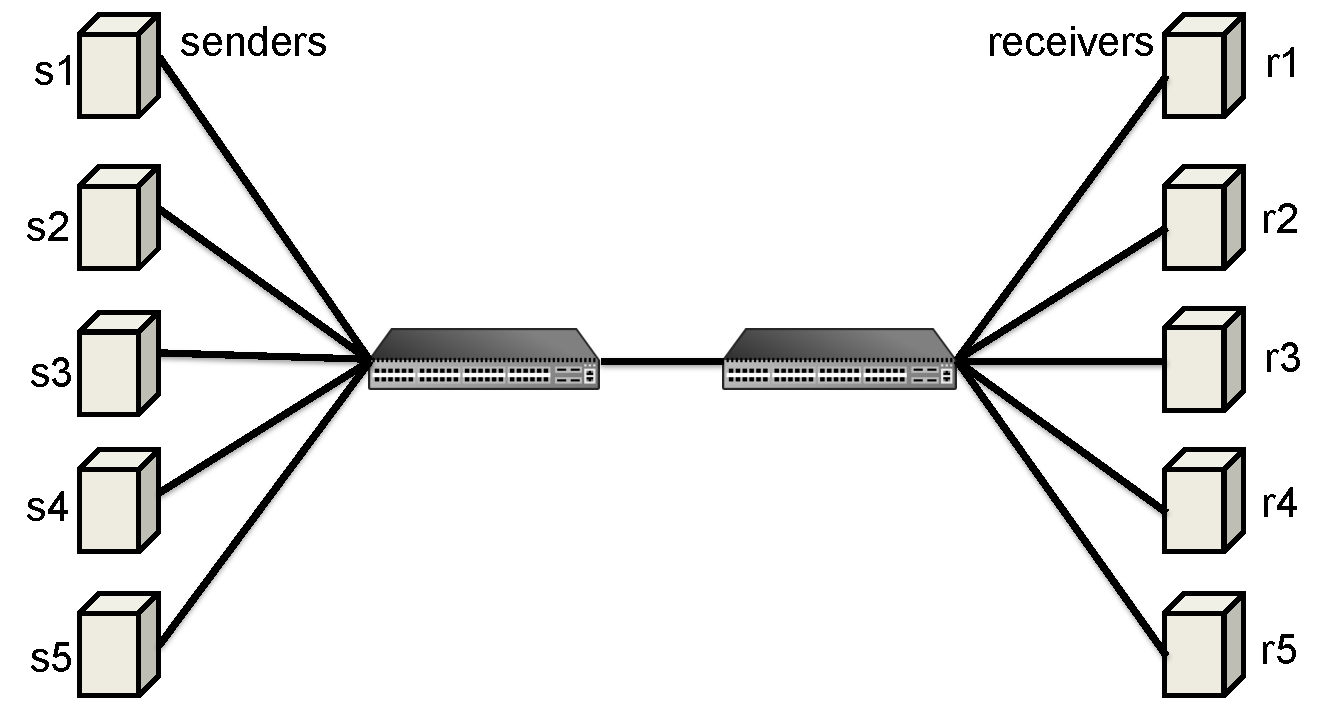
\includegraphics[width=0.7\textwidth]{acdctcp/figures/dumbbell_topology.pdf}
                \caption{Dumbbell topology.}
                \label{dumbbell_topology}
        \end{subfigure}
        \begin{subfigure}[b]{0.45\textwidth}
                \centering
                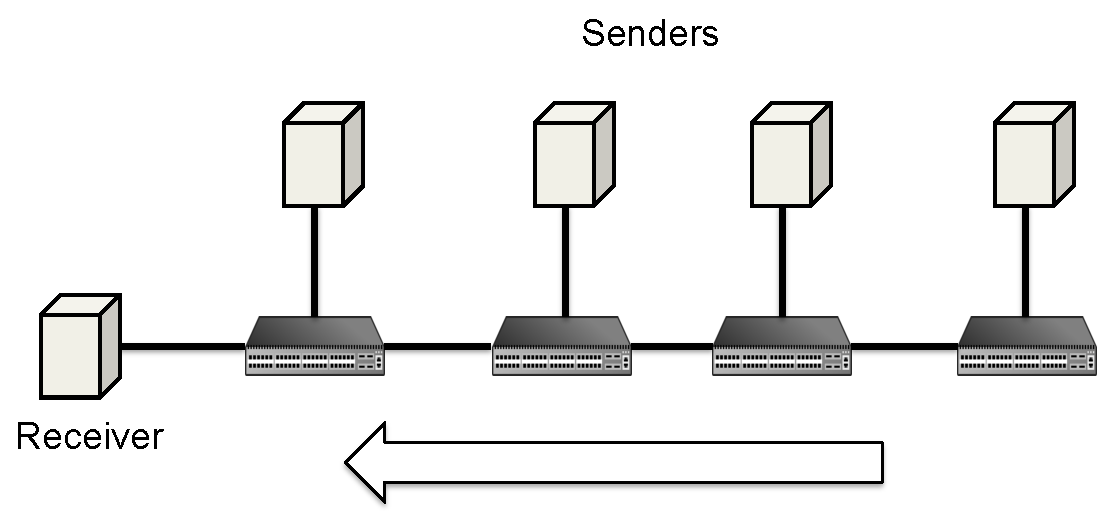
\includegraphics[width=0.7\textwidth]{acdctcp/figures/parkinglot_topology.pdf}
                \caption{Multi-hop, multi-bottleneck (parking lot) topology.}
                \label{parkinglot_topology}
        \end{subfigure}
        \caption{Experiment topologies.}
        \label{microbenchmarks_topology}
\end{figure}

%%%% topology %%%

\begin{figure}[!t]
        \centering
  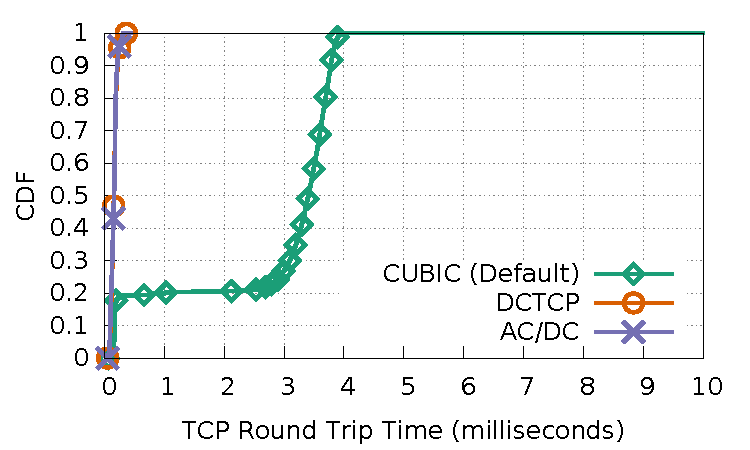
\includegraphics[width=0.5\textwidth]{acdctcp/figures/convergence/flowcontrolOFF_sockperf/convergence_test_sockperf.pdf}
        \caption{RTT of schemes on dumbbell topology.}
        \label{sockperf_convergence}
\end{figure}

We first evaluate \acdc{}'s performance using a set of microbenchmarks.
The microbenchmarks are conducted on topologies shown in Figure~\ref{microbenchmarks_topology}.

\tightparagraph{Canonical topologies}
We aim to understand the performance of our scheme on two simple topologies.
First, one long-lived flow is started per server pair ($s_i$ to $r_i$) in Figure~\ref{dumbbell_topology}. 
The average per-flow throughput of \acdc{}, DCTCP and CUBIC are all 1.98Gbps.
Figure~\ref{sockperf_convergence} is a CDF of the RTT
from the same test. Here, increases in RTT are caused by queueing delay in the switch.
~\acdc{} achieves comparable RTT with DCTCP and significantly outperforms CUBIC.

Second, each sender in Figure~\ref{parkinglot_topology} starts a long-lived
flow to the receiver. Each flow traverses a different number of 
bottleneck links. CUBIC has an average per-flow throughput of 2.48Gbps with
a Jain's fairness index of 0.94, and
both DCTCP and \acdc{} obtain an average throughput of 2.45Gbps with a
fairness index of 0.99. 
The 50$^{th}$ and 99.9$^{th}$ percentile RTT for
\acdc{} (DCTCP, CUBIC) are 124$\mu$s (136$\mu$s, 3.3ms) and
279$\mu$s (301$\mu$s, 3.9ms), respectively.

%TCP-Bolt~\cite{stephens2014practical} and DCQCN~\cite{zhu2015congestion} found
%that Data Center Bridging (DCB) can have throughput unfairness and 
%increased queueing (bufferbloat) issues and such issues can be solved by utilizing
%ECN (like DCTCP). We anticipate our scheme can also work in DCB.

%%how close our RWND is to DCTCP's CWND
\begin{figure}[!t]
        \centering
        \begin{subfigure}[b]{0.45\textwidth}
                \centering
                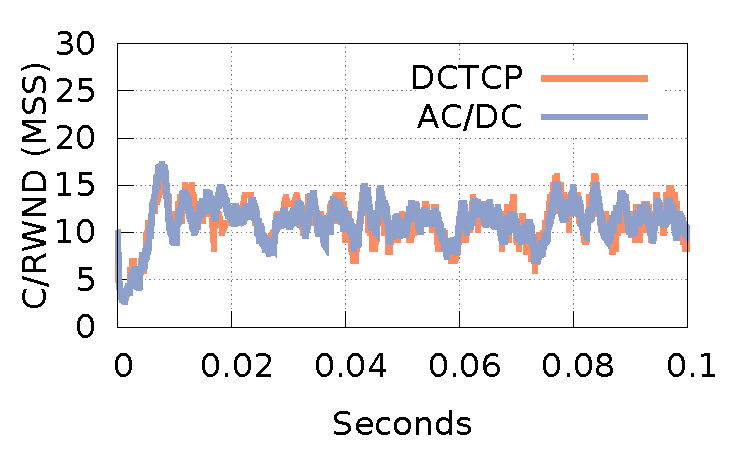
\includegraphics[width=\textwidth]{acdctcp/figures/cwnd_rwnd/newpara_refine/mtu1500_5flows_1/measure_cwnd_rwnd_gap_15k_5flows_0sec_100msec.pdf}
                \caption{First 100 ms of a flow.}
                \label{cwnd_rwnd_1500}
        \end{subfigure}
        \begin{subfigure}[b]{0.45\textwidth}
                \centering
                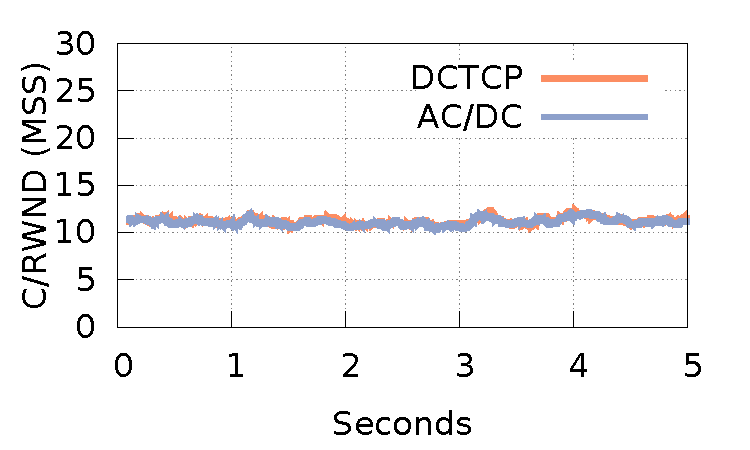
\includegraphics[width=\textwidth]{acdctcp/figures/cwnd_rwnd/moving-ave/measure_cwnd_rwnd_gap_15k_5flows_ave100.pdf}
                \caption{Moving average.}
                \label{cwnd_rwnd_1500_ave}
        \end{subfigure}

        \caption{~\acdc{}'s \rwnd{} tracks DCTCP's~\cwnd{} (1.5KB MTU).}
        \label{compare_cwnd_rwnd}
\end{figure}



%%who limits TCP throughput, CWND or RWND? CUBIC
\begin{figure}[!t]
        \centering
        \begin{subfigure}[b]{0.45\textwidth}
                \centering
                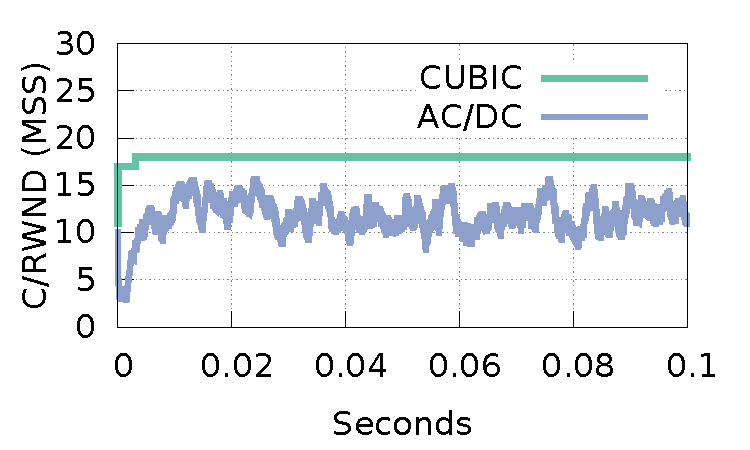
\includegraphics[width=\textwidth]{acdctcp/figures/cwnd_rwnd2/mtu1500_cubic/cubic_measure_cwnd_rwnd_gap_15k_5flows_0sec_100msec.pdf}
                \caption{Starting from 0 sec.}
                \label{who_limits_cwnd_rwnd_1500_0sec}
        \end{subfigure}
        \begin{subfigure}[b]{0.45\textwidth}
                \centering
                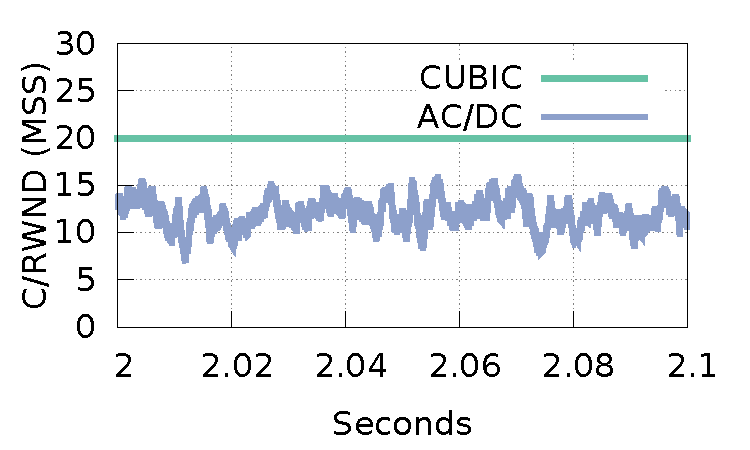
\includegraphics[width=\textwidth]{acdctcp/figures/cwnd_rwnd2/mtu1500_cubic/cubic_measure_cwnd_rwnd_gap_15k_5flows_2sec_100msec.pdf}
                \caption{Starting from 2 sec.}
                \label{who_limits_cwnd_rwnd_1500_2sec}
        \end{subfigure}
%        \begin{subfigure}[b]{0.225\textwidth}
%                \centering
%                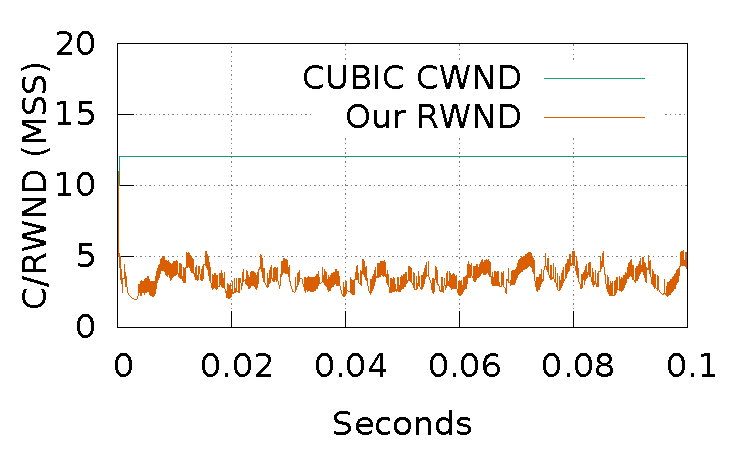
\includegraphics[width=\textwidth]{acdctcp/figures/cwnd_rwnd2/mtu9000_cubic/cubic_measure_cwnd_rwnd_gap_9k_5flows_0sec_100msec.pdf}
%                \caption{MTU9000: first 100 msec starting from second 0.}
%                \label{who_limits_cwnd_rwnd_9000_0sec}
%        \end{subfigure}
%        \begin{subfigure}[b]{0.225\textwidth}
%                \centering
%                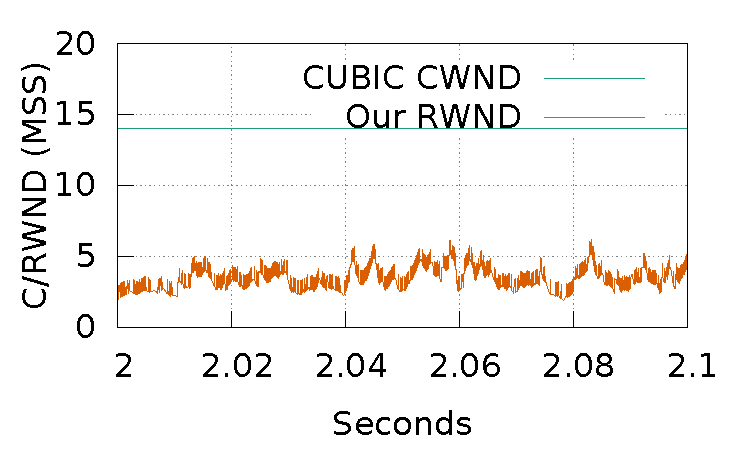
\includegraphics[width=\textwidth]{acdctcp/figures/cwnd_rwnd2/mtu9000_cubic/cubic_measure_cwnd_rwnd_gap_9k_5flows_2sec_100msec.pdf}
%                \caption{MTU9000: first 100 msec starting from second 2.}
%                \label{who_limits_cwnd_rwnd_9000_2sec}
%        \end{subfigure}
        \caption{Who limits TCP throughput when~\acdc{} is run with CUBIC? (1.5 KB MTU)}
        \label{who_limits_compare_cwnd_rwnd}
\end{figure}

\begin{figure}[!t]
        \centering
  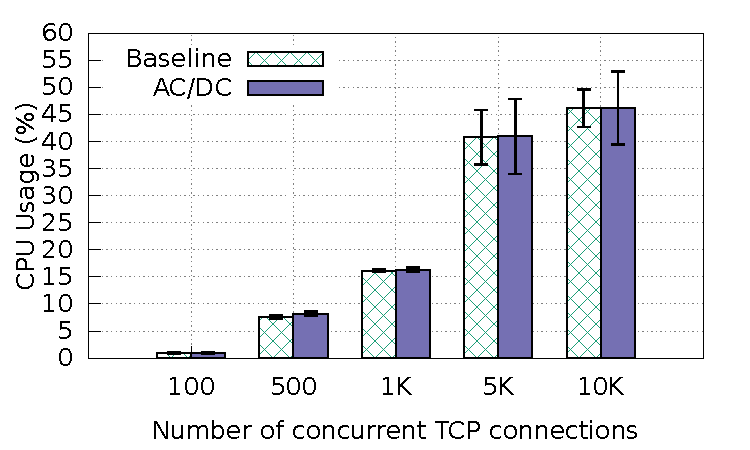
\includegraphics[width=0.5\textwidth]{acdctcp/figures/overhead/sender_15k_compare_cpu_witherrbar.pdf}
        \caption{CPU overhead: sender side (1.5KB MTU).}
        \label{cpu_overhead_sender_15k}
\end{figure}

\begin{figure}[!t]
        \centering
  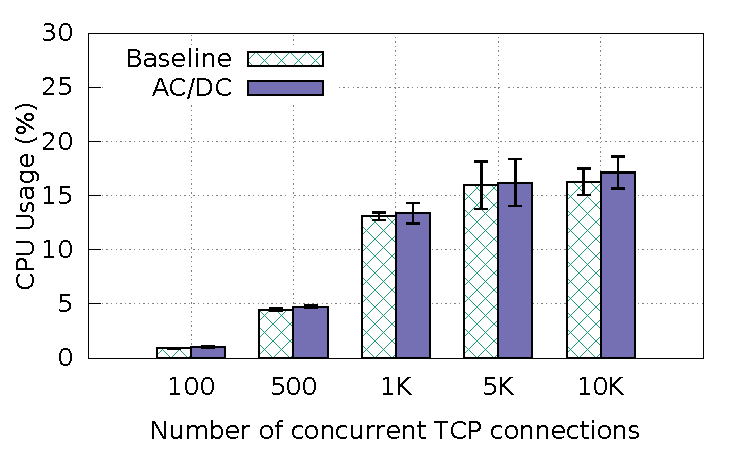
\includegraphics[width=0.5\textwidth]{acdctcp/figures/overhead/receiver_15k_compare_cpu_witherrbar.pdf}
        \caption{CPU overhead: receiver side (1.5KB MTU).}
        \label{cpu_overhead_receiver_15k}
\end{figure}


\begin{figure}[!t]
        \centering
  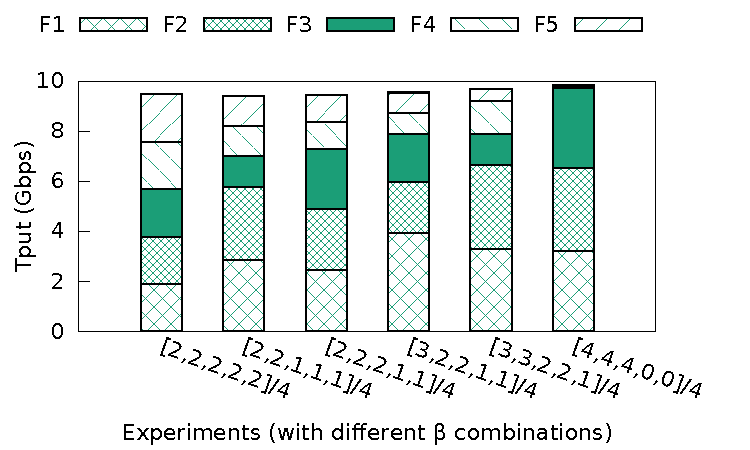
\includegraphics[width=0.5\textwidth]{acdctcp/figures/qos/qos_stacked.pdf}
        \caption{\crs{\acdc{} provides differentiated throughput via QoS-based CC. $\beta$ values are defined on a 4-point scale.}}
        \label{cc-qos}
\end{figure}

\tightparagraph{Tracking window sizes}
Next, we aim to understand how accurately~\acdc{} tracks DCTCP's performance at a finer level. The host's TCP
stack is set to DCTCP and our scheme runs in the vSwitch.
We repeat the experiment in Figure~\ref{dumbbell_topology} and measure the~\rwnd{} calculated by~\acdc{}. Instead
of over-writing the~\rwnd{} value in the ACKs, we simply log the value to a file. Thus, congestion is enforced by DCTCP
and we can capture DCTCP's~\cwnd{} by using {\tt tcpprobe}~\cite{tcp-probe}. We align the~\rwnd{} and~\cwnd{} values by timestamps and sequence
numbers and show a timeseries in Figure~\ref{compare_cwnd_rwnd}. Figure~\ref{cwnd_rwnd_1500} shows both windows for the
first 100 ms of a flow and shows that~\acdc{}'s calculated window closely tracks DCTCP's. Figure~\ref{cwnd_rwnd_1500_ave} 
shows the windows over a 100ms moving average are also similar. This suggests it is possible to accurately recreate congestion
control in the vSwitch.~\crs{These results are obtained with 1.5KB MTU. Trends for 9KB MTU are similar but the window sizes are smaller}.

We were also interested to see how often~\acdc{}'s congestion window takes effect. We rerun the experiment~\crs{(MTU is still 1.5KB)}, but set
the host TCP stack to CUBIC. The~\rwnd{} computed by~\acdc{} is both written into the ACK and logged to a file. We again
use {\tt tcpprobe} to measure CUBIC's~\cwnd{}. Figure~\ref{who_limits_compare_cwnd_rwnd} is a timeseries (one graph from the
start of the experiment and one graph 2 seconds in) that shows~\acdc{}'s
congestion control algorithm is indeed the limiting factor.
In the absence of loss or ECN markings, traditional TCP stacks do not severely reduce~\cwnd{} and thus
\acdc{}'s~\rwnd{} becomes the main enforcer of a flow's congestion control. Because DCTCP 
is effective at reducing loss and~\acdc{} hides ECN feedback from the host TCP stack,
~\acdc{}'s enforcement is applied often.
%As before, 9KB MTU results showed similar trends.

%
%\begin{figure}[!htb]
%        \centering
%  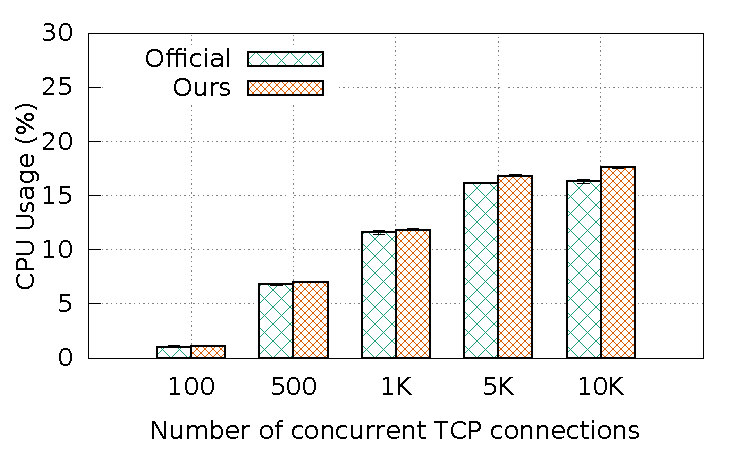
\includegraphics[width=0.45\textwidth]{acdctcp/figures/overhead/sender_9k_compare_cpu_witherrbar.pdf}
%        \caption{CPU overhead: sender side (9K MTU). The 10G NIC is saturated when there are more than 1K TCP connections.
%		CPU usage refers to the CPU usage of the whole server (12 Intel(R) Xeon(R) CPU E5649@2.53GHz processors)
%                measured by ``sar (sysstat)''.}
%        \label{cpu_overhead_sender_9k}
%\end{figure}
%
%\begin{figure}[!htb]
%        \centering
%  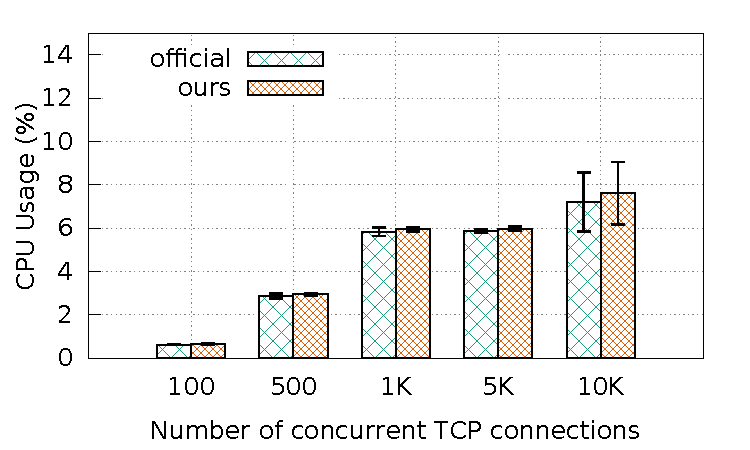
\includegraphics[width=0.45\textwidth]{acdctcp/figures/overhead/receiver_9k_compare_cpu_witherrbar.pdf}
%        \caption{CPU overhead: receiver side (9K MTU). The 10G NIC is saturated when there are more than 1K TCP connections.
%		CPU usage refers to the CPU usage of the whole server (12 Intel(R) Xeon(R) CPU E5649@2.53GHz processors)
%                measured by ``sar (sysstat)''}
%        \label{cpu_overhead_receiver_9k}
%\end{figure}
%

\tightparagraph{CPU overhead}
We measure the CPU overhead of~\acdc{} by connecting two servers to a single switch. 
Multiple simultaneous TCP flows are started from one server to the other and the total CPU utilization
is measured on the sender and receiver using {\tt sar}. Each flow is given time to perform the TCP handshake
and when all are connected, each TCP client sends with a demand of 10 Mbps by sending 128KB bursts every 100 milliseconds (so 1,000 connections saturate the 10 Gbps link). 
The~\crs{system-wide} CPU overhead of~\acdc{} compared to the~\crs{system-wide} CPU overhead of baseline (\ie{}, just OVS) 
is shown for the sender in Figure~\ref{cpu_overhead_sender_15k}
 and the receiver in Figure~\ref{cpu_overhead_receiver_15k}.~\crs{Error bars show standard deviation over 50 runs.
While~\acdc{} increases CPU usage in all cases, the increase is negligible. The largest difference is less than one percentage point: 
the baseline and~\acdc{} have 16.27\% and 17.12\% utilization, respectively for 10K flows at the receiver.
%Even when scaling to 
%10,000 connections, the CPU overhead of our scheme is less than 1\%.
The results are shown with 1.5KB MTU because smaller packets incur higher overhead. Note experiments with 9KB MTU have similar trends.}
%https://en.wikipedia.org/wiki/Relative_change_and_difference
%https://www.mathsisfun.com/percentage-points.html


%%% other TCP variants %%%
\begin{table*}[!t]
\tiny
\begin{center}
\begin{tabular}{ |c|c|c|c|c|c|c|c|c| }
 \hline
 \multirow{2}{*}{CC Variants} & \multicolumn{2}{|c|}{50$^{th}$ percentile RTT ($\mu$s)} & \multicolumn{2}{|c|}{99$^{th}$ percentile RTT ($\mu$s)} & \multicolumn{2}{|c|}{Avg Tput (Gbps)} & \multicolumn{2}{|c|}{Fairness Index}\\
 \cline{2-9}
       &  mtu=1.5KB & mtu=9KB & mtu=1.5KB & mtu=9KB & mtu=1.5KB & mtu=9KB & mtu=1.5KB & mtu=9KB\\
 \hline
 \hline
 CUBIC* &  3232     &   3448    &   3641     &  3865     &   1.89    & 1.98   &  0.85   &   0.98\\
 DCTCP* &  128      &   142    &   232    &   259    &   1.89    &   1.98  &  0.99    &   0.99\\
 \hline
 \hline
 CUBIC &   128     &   142    &    231    &   252    &   1.89    &  1.98   &  0.99    &  0.99 \\
 Reno  &   120     &   149    &    235    &   248    &   1.89    &  1.97   &  0.99    &  0.99 \\
DCTCP  &   129     &   149    &    232    &   266    &   1.88    &  1.98   &  0.99    &  0.99 \\
Illinois  &   134     &   152    &    215    &  262     &   1.89    &  1.97   &  0.99    &  0.99 \\
HighSpeed  &   119     &  147     &    224    &  252     &   1.88    & 1.97    &  0.99    & 0.99  \\
 Vegas  &   126     &   143    &    216    &    251   &   1.89    &  1.97   &  0.99    &  0.99 \\

 \hline

\end{tabular}
\caption{\acdc{} works with many congestion control variants.~\crs{Legend:}
        CUBIC*: CUBIC + standard OVS, switch WRED/ECN marking off.
        DCTCP*: DCTCP + standard OVS, switch WRED/ECN marking on.
        Others: different CCs + \acdc{}, switch WRED/ECN marking on.}
\label{other_cc_variants}
\end{center}
\end{table*}

%%%convergence %%%
\begin{figure*}[!t]
        \centering
        \begin{subfigure}[b]{0.3\textwidth}
                \centering
                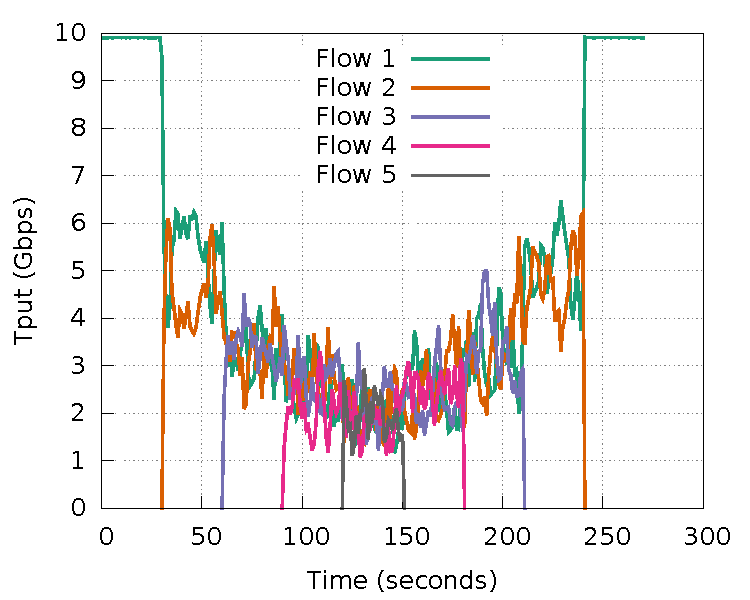
\includegraphics[width=\textwidth]{acdctcp/figures/convergence/flowcontrolOFF/tcp_flowcontrolOFF_convergence.pdf}
                \caption{CUBIC convergence test.}
                \label{cubic_convergence}
        \end{subfigure}
        \begin{subfigure}[b]{0.3\textwidth}
                \centering
                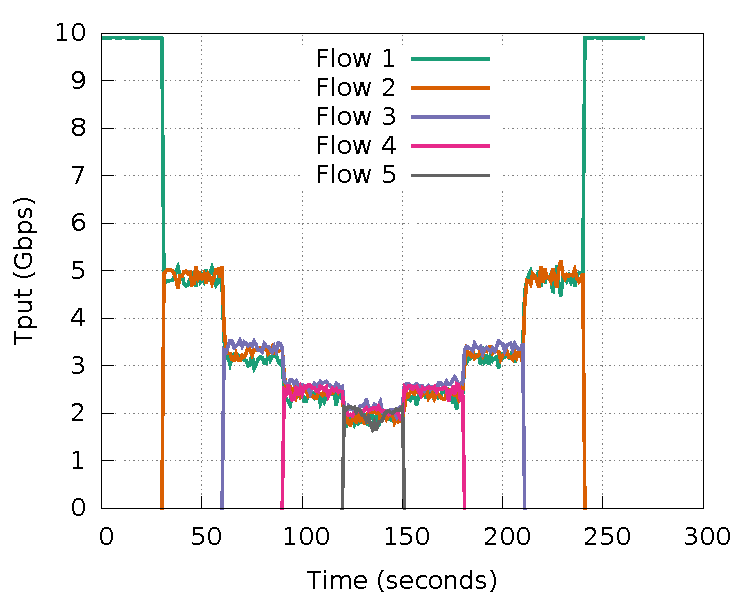
\includegraphics[width=\textwidth]{acdctcp/figures/convergence/flowcontrolOFF/dctcp_flowcontrolOFF_convergence.pdf}
                \caption{DCTCP convergence test.}
                \label{dctcp_convergence}
        \end{subfigure}
        \begin{subfigure}[b]{0.3\textwidth}
                \centering
                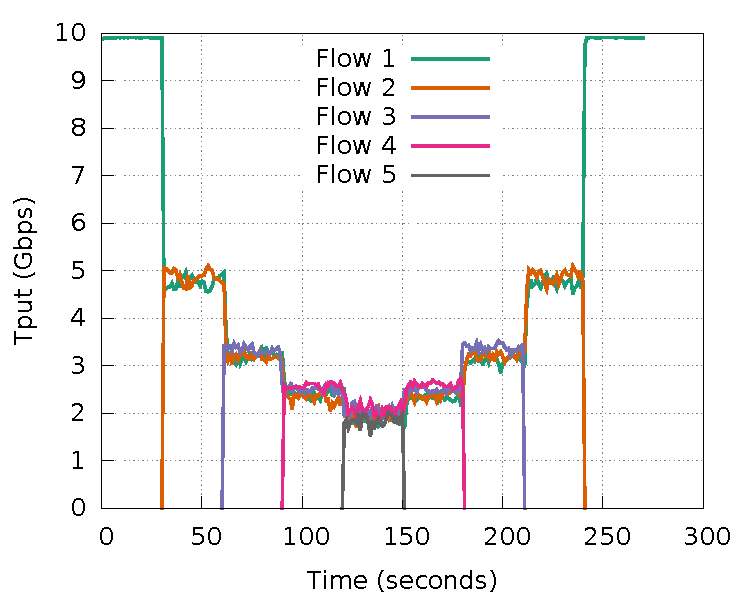
\includegraphics[width=\textwidth]{acdctcp/figures/convergence/flowcontrolOFF/ovsdctcp_flowcontrolOFF_convergence.pdf}
                \caption{\acdc{} convergence test.}
                \label{ovsdctcp_convergence}
        \end{subfigure}
        \caption{~\crs{Convergence tests: flows are added, then removed, every 30 secs.~\acdc{} performance matches DCTCP.}}
        \label{convergence_test}
\end{figure*}


\tightparagraph{~\acdc{} flexibility}~\acdc{} aims to provide a degree of control and flexibility over tenant TCP stacks. 
We consider two cases.
First,~\acdc{} should work effectively, regardless of the tenant TCP stack.
Table~\ref{other_cc_variants} shows the performance of our scheme when various TCP congestion control algorithms
are configured on the host. Data is collected over 10 runs lasting 20 seconds each on the dumbbell topology (Figure~\ref{dumbbell_topology}). 
The first two rows of the table, CUBIC* and DCTCP*, show the performance of each stack with an 
unmodified OVS. The next six rows show the performance of a given host stack with~\acdc{} running DCTCP in OVS.
The table shows~\acdc{} can effectively track the performance of DCTCP*, meaning 
it is compatible with popular delay-based (Vegas) and loss-based (Reno, CUBIC, etc) stacks.

Second,~\acdc{} enables an administrator to assign different 
congestion control algorithms on a per-flow basis. 
%For example, congestion control algorithms shown to optimize WAN performance, 
%such as Compound TCP~\cite{tan2006compound}, can be employed on front-end
%web server traffic, while DCTCP can be used for intra-DC back-end traffic.
For example,~\acdc{} can provide the flexibility to implement QoS through differentiated congestion control. 
We fix the host TCP stack to CUBIC and alter~\acdc{}'s congestion control for each flow
by setting the $\beta$ value (in Equation~\ref{eqn:cc-qos}) for each flow in the dumbbell topology. 
Figure~\ref{cc-qos} shows the throughput achieved by each flow, 
along with its $\beta$ setting.~\acdc{} is 
able to provide relative bandwidth allocation to each flow based on $\beta$. 
Flows with the same $\beta$ value get similar throughputs and flows with higher $\beta$ values 
obtain higher throughput.
The latencies (not shown) remain consistent with
previous results.


%%%coexistence %%%
\begin{figure}[!t]
        \centering
        \begin{subfigure}[b]{0.45\textwidth}
                \centering
                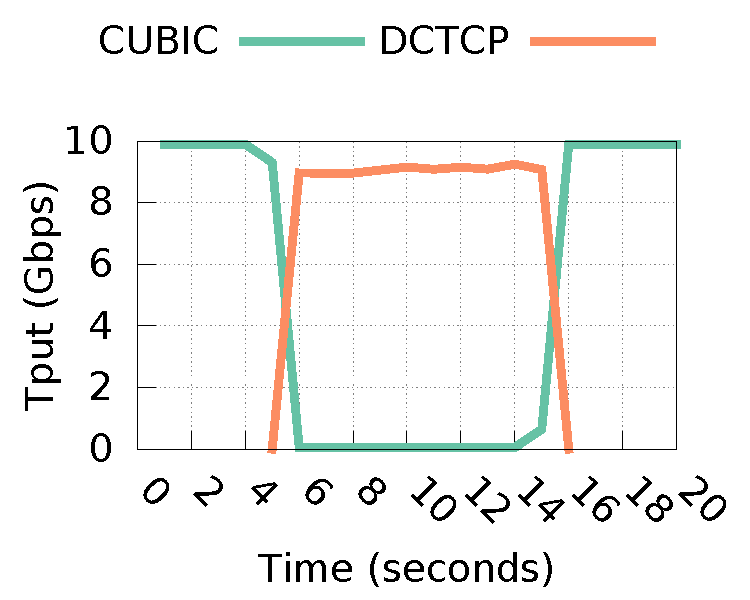
\includegraphics[width=\textwidth]{acdctcp/figures/micro2flows/coexitence/cubic_dctcp_coexistence_official.pdf}
                \caption{Default.}
                \label{coexistence_tput_ovs}
        \end{subfigure}
        \begin{subfigure}[b]{0.45\textwidth}
                \centering
                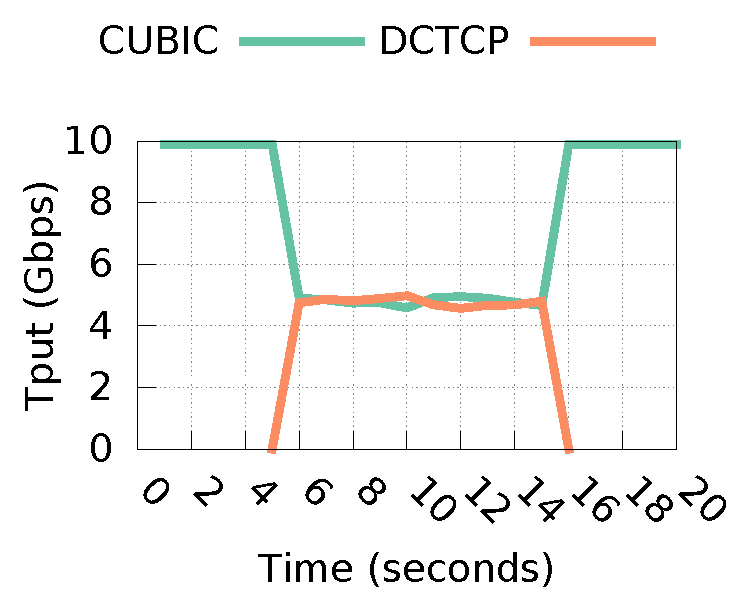
\includegraphics[width=\textwidth]{acdctcp/figures/micro2flows/coexitence/cubic_dctcp_coexistence_acdctcp.pdf}
                \caption{\acdc{}.}
                \label{coexistence_tput_ovsdctcp}
        \end{subfigure}
        \caption{(a) CUBIC gets little throughput when competing with DCTCP.
		 (b) With \acdc{}, CUBIC and DCTCP flows get fair share.}
        \label{coexistence_tput}
\end{figure}

\begin{figure}[!t]
        \centering
  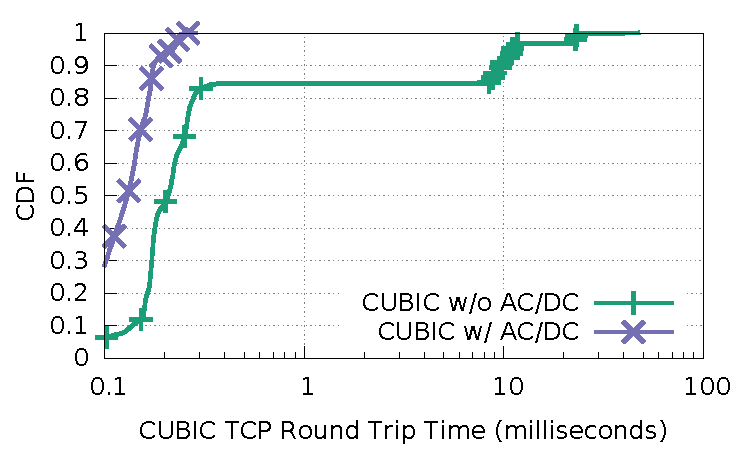
\includegraphics[width=0.5\textwidth]{acdctcp/figures/micro2flows/coexitence/sockperf_and_droprate/coexistence_sockperf.pdf}
        \caption{CUBIC experiences high RTT when competing with DCTCP.~\acdc{} fixes this issue.}
        \label{coexistence_sockperf_droprate}
\end{figure}

\begin{figure}[!t]
        \centering
%        \begin{subfigure}[b]{0.24\textwidth}
%                \centering
%                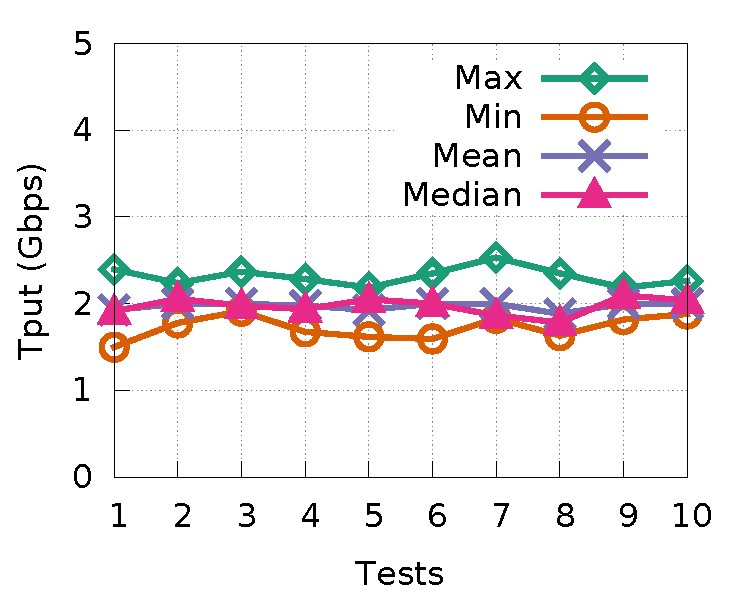
\includegraphics[width=\textwidth]{acdctcp/figures/tput_fairness/default_all_cubic_tput.pdf}
%                \caption{All CUBIC.}
%                \label{fairness_all_cubic}
%        \end{subfigure}
%        \begin{subfigure}[b]{0.24\textwidth}
%                \centering
%                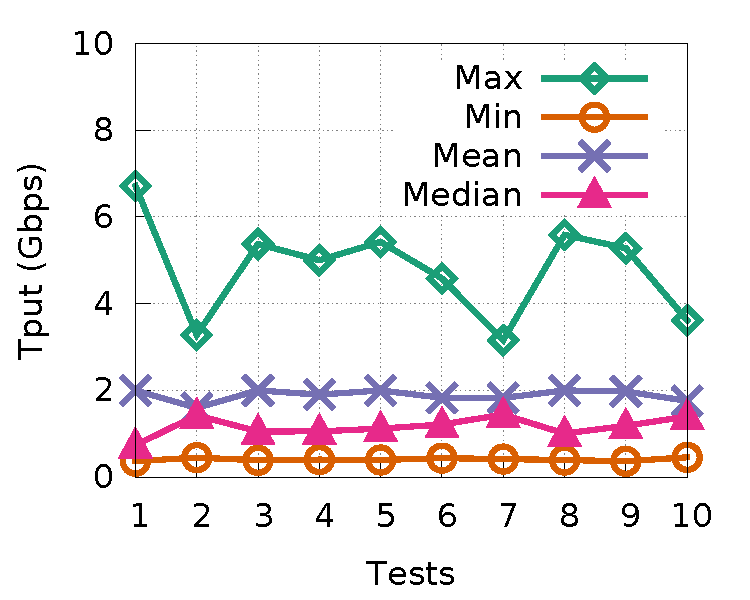
\includegraphics[width=\textwidth]{acdctcp/figures/tput_fairness/default_5CC_tput.pdf}
%                \caption{5 different CCs.}
%                \label{fairness_5CC}
%        \end{subfigure}
        \begin{subfigure}[b]{0.45\textwidth}
                \centering
                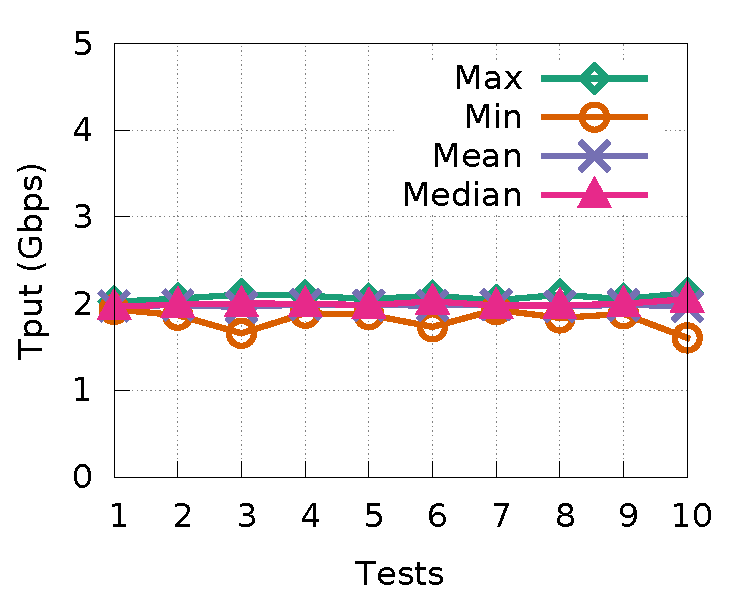
\includegraphics[width=\textwidth]{acdctcp/figures/tput_fairness/ecn_all_dctcp_tput.pdf}
                \caption{All DCTCP.}
                \label{fairness_5CC_with_dctcp}
        \end{subfigure}
        \begin{subfigure}[b]{0.45\textwidth}
                \centering
                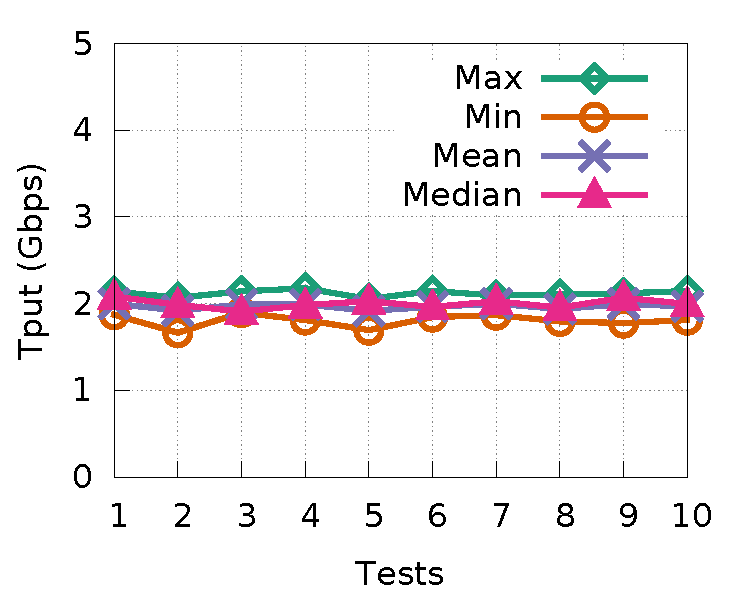
\includegraphics[width=\textwidth]{acdctcp/figures/tput_fairness/liquid_5CC_tput.pdf}
                \caption{5 different CCs (\acdc{}).}
                \label{fairness_5CC_with_ours}
        \end{subfigure}
	\caption{~\crs{\acdc{} improves fairness when VMs implement different CCs. DCTCP performance shown for reference.}} 
 	\label{tput_fairness_coexistence}
\end{figure}	


\tightparagraph{Fairness}
Three different experiments are used to demonstrate fairness. First, we show~\acdc{} can mimic DCTCP's 
behavior in converging to fair throughputs. We repeat the experiment originally performed 
by Alizadeh~\cite{alizadeh2011data} and Judd~\cite{judd2015nsdi} by 
adding a new flow every 30 seconds on a bottleneck link and then reversing the process. 
The result is shown in Figure~\ref{convergence_test}.
Figure~\ref{cubic_convergence} shows CUBIC's problems converging to fair allocations.
Figures~\ref{dctcp_convergence}
and~\ref{ovsdctcp_convergence} show DCTCP and~\acdc{} performance, respectively.~\acdc{} tracks DCTCP's behavior.
CUBIC's drop rate is 0.17\% while DCTCP's and \acdc{}'s is 0\%. 
%Note that as mentioned in~\cite{judd2015nsdi}, CUBIC's 
%performance can be improved by manually altering the socket buffer size, 
%but let applications sizing it in practice is hard. DCTCP, and thus
%our scheme, do not need this optimization, 
%thus demonstrating one additional benefit of our approach.

The second experiment is also repeated from Judd's paper~\cite{judd2015nsdi}. 
ECN-capable and non-ECN-capable flows do not coexist well because switches
drop non-ECN packets when the queue length is larger than the marking threshold. Figure~\ref{coexistence_tput_ovs}
shows the throughput of CUBIC suffers when CUBIC (with no ECN) and DCTCP (with ECN) traverse the same bottleneck link.
Figure~\ref{coexistence_tput_ovsdctcp} shows~\acdc{} alleviates this problem 
because it forces all flows to become ECN-capable.
Figure~\ref{coexistence_sockperf_droprate} shows CUBIC's RTT is extremely high
in the first case because switches drop non-ECN packets (the loss rate is 0.18\%) and thus
there is a significant number of retransmissions. However,~\acdc{} eliminates 
this issue and reduces latency.
%\emph{\acdc{} makes low latency possible in production data center networks where
%incremental deployment is the norm and transport diversity must be supported}.

The last experiment examines the impact of having multiple TCP stacks on the same fabric. 
Five flows with different congestion control algorithms (CUBIC, Illinois, HighSpeed, New Reno and Vegas) are started
on the dumbbell topology. This is the same experiment as in Figure~\ref{tput_unfair}.
Figure~\ref{fairness_5CC_with_dctcp} shows what happens if all
flows are configured to use DCTCP and Figure~\ref{fairness_5CC_with_ours} shows when
the five different stacks traverse~\acdc{}. We can see~\acdc{} closely tracks the ideal case of
all flows using DCTCP, and~\acdc{} and DCTCP provide better fairness than all CUBIC (Figure~\ref{unfairness_all_cubic}).
%The median and 99.9\% TCP RTTs for all CUBIC, 5 different CCs, 5 different CCs with
%our logic and all DCTCP are: 3.5 ms, 3.9 ms; 3.4 ms, 4.0 ms; 146 $\mu$s, 306 $\mu$s;
%147 $\mu$s, 317 $\mu$s. Both~\acdc{} and DCTCP obtain a Jain's fairness index greater than 0.99.


\iffalse
\tightparagraph{Different MTU sizes}
We set MTU size to 1500 bytes and run the tests on the dumbbell topology (Figure~\ref{dumbbell_topology})
with 5 flows competing for
a 10G bottleneck link. \acdc{} gets 1.87Gbps average flow throughput. DCTCP gets 1.88Gbps average flow throughput. 
Both have a Jain's fairness index greater than 0.99. TCP CUBIC gets 1.89 average flow throughput and a fairness index of 0.85.
The 50$^{th}$ and 99.9$^{th}$ percentile TCP RTT for \acdc{} (DCTCP, CUBIC) are 139$\mu$s (136$\mu$s, 3.2ms) and
359$\mu$s (342$\mu$s, 3.7ms), respectively.
~\eric{KEQIANG: please look at this paragraph and see how it fits in the
"Canonical Topologies" paragraph. Our numbers should be consistent. We can 
remove this paragraph afterwards.}
\fi

\subsection{Macrobenchmarks}
\label{macro}

%%%%%%%%%%using figures to present incast: tput, fariness, droprate, TCP RTT
\begin{figure}[!t]
        \centering
        \begin{subfigure}[b]{0.45\textwidth}
                \centering
                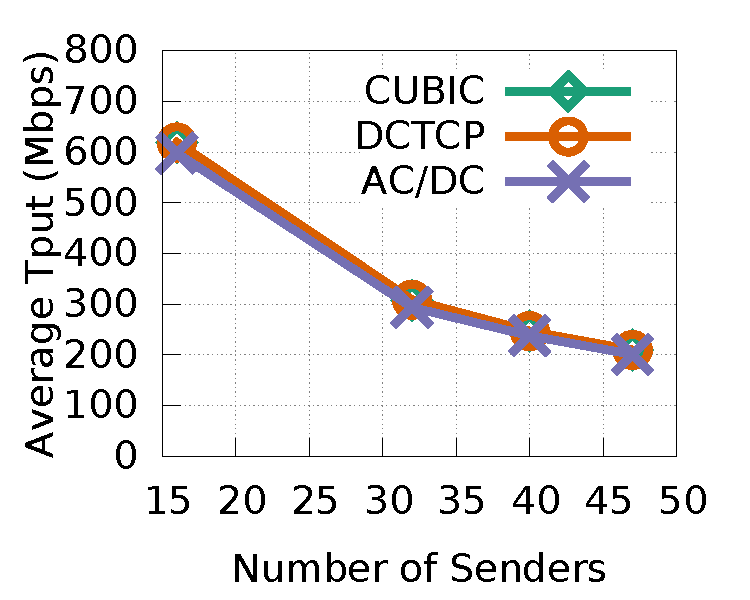
\includegraphics[width=\textwidth]{acdctcp/figures/incast/plots9k/incast_tput_vary_sender.pdf}
                \caption{Average throughput.}
                \label{incast_9k_tput}
        \end{subfigure}
        \begin{subfigure}[b]{0.45\textwidth}
                \centering
                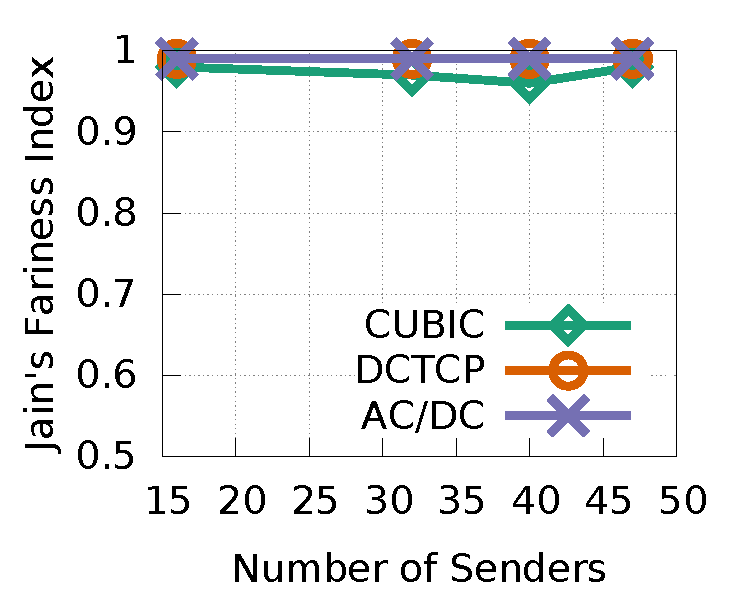
\includegraphics[width=\textwidth]{acdctcp/figures/incast/plots9k/incast_fairness_vary_sender.pdf}
                \caption{Fairness.}
                \label{incast_9k_fariness}
        \end{subfigure}
        \caption{Many to one incast: throughput and fairness.}
        \label{incast_9k_tput_fairness}
\end{figure}

\begin{figure*}[!t]
        \centering
        \begin{subfigure}[b]{0.3\textwidth}
                \centering
                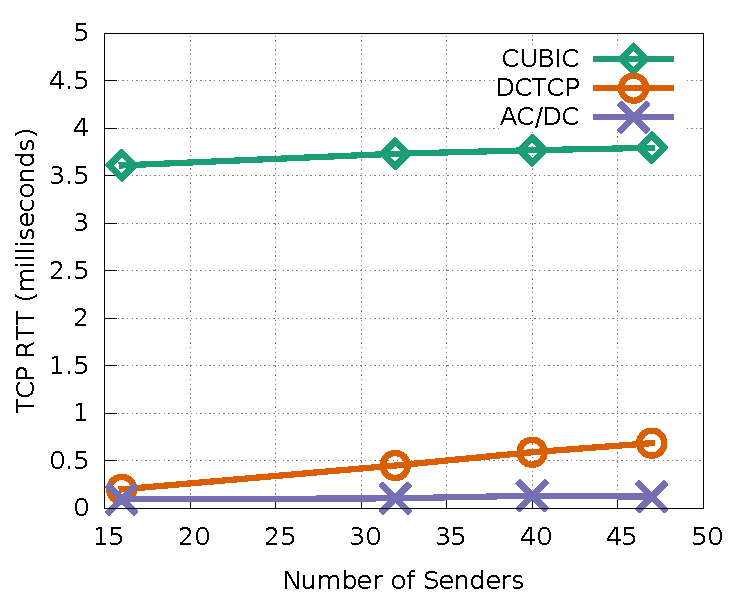
\includegraphics[width=\textwidth]{acdctcp/figures/incast/plots9k/incast_sockperf50th_vary_sender.pdf}
                \caption{50$^{th}$ percentile RTT.}
                \label{incast_9k_50th_sockperf}
        \end{subfigure}
        \begin{subfigure}[b]{0.3\textwidth}
                \centering
                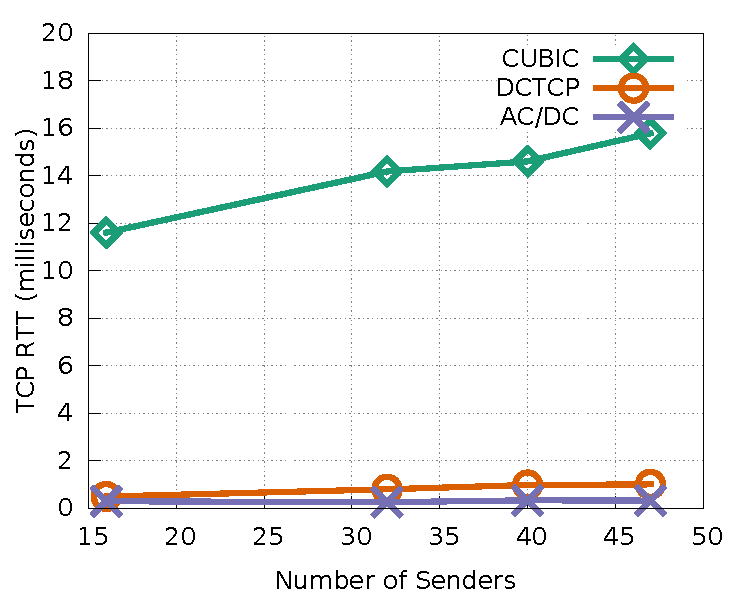
\includegraphics[width=\textwidth]{acdctcp/figures/incast/plots9k/incast_sockperf999th_vary_sender.pdf}
                \caption{99.9$^{th}$ percentile RTT.}
                \label{incast_9k_999th_sockperf}
        \end{subfigure}
        \begin{subfigure}[b]{0.3\textwidth}
                \centering
                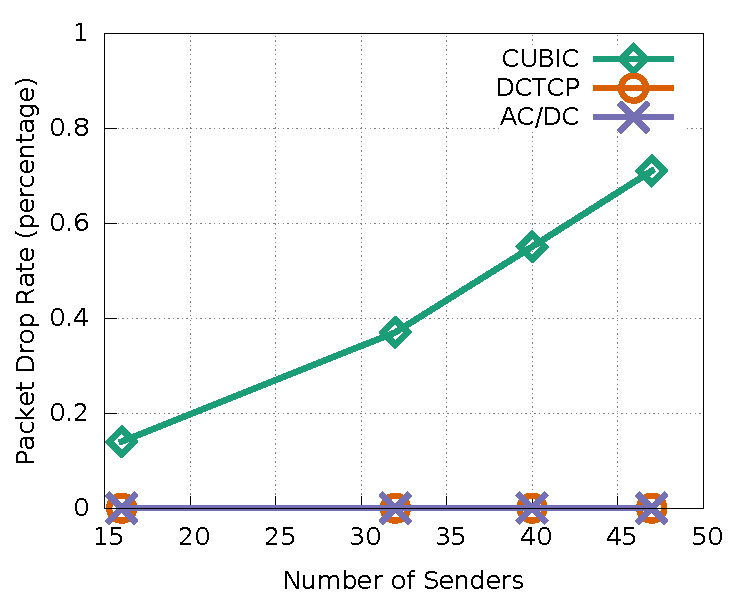
\includegraphics[width=\textwidth]{acdctcp/figures/incast/plots9k/incast_droprate_vary_sender.pdf}
                \caption{Packet drop rate.}
                \label{incast_9k_droprate}
        \end{subfigure}
        \caption{Many to one incast: RTT and packet drop rate.\crs{~\acdc{} can reduce DCTCP's RTT by limiting window sizes.}}
        \label{incast_9k_sockperf_droprate}
\end{figure*}


\begin{figure}[!t]
        \centering
  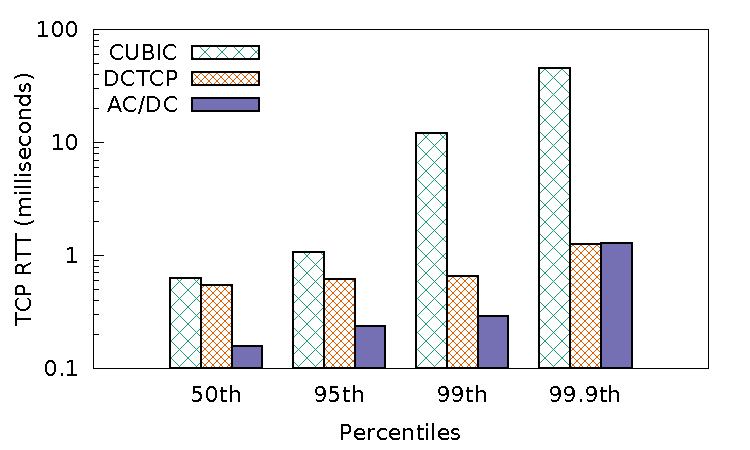
\includegraphics[width=0.5\textwidth]{acdctcp/figures/incast/pressure/incast_pressure_compare_sockperf.pdf}
        \caption{TCP RTT when almost all ports are congested.}
        \label{sockperf_pressure_incast}
\end{figure}

%
%

\iffalse
\begin{figure*}[!t]
        \centering
        \begin{subfigure}[b]{0.45\textwidth}
                \centering
                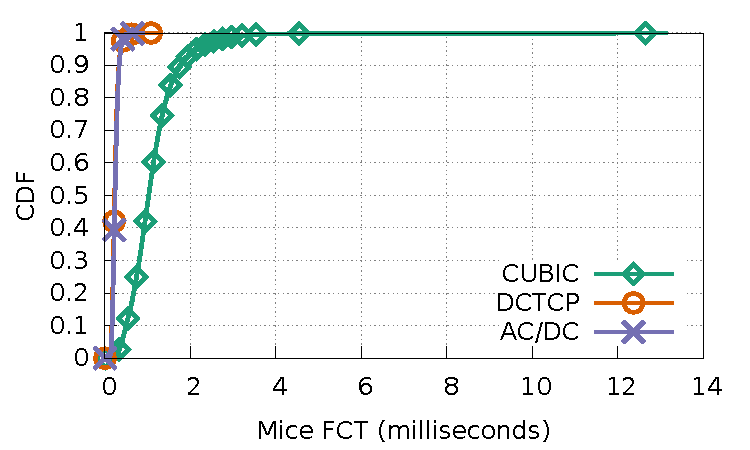
\includegraphics[width=\textwidth]{acdctcp/figures/macro_benchmarks/macro_4stride/stride4_mice16KB_fct.pdf}
                \caption{Mice flow completion times.}
                \label{macro_4stride_mice_fct}
        \end{subfigure}
        \begin{subfigure}[b]{0.45\textwidth}
                \centering
                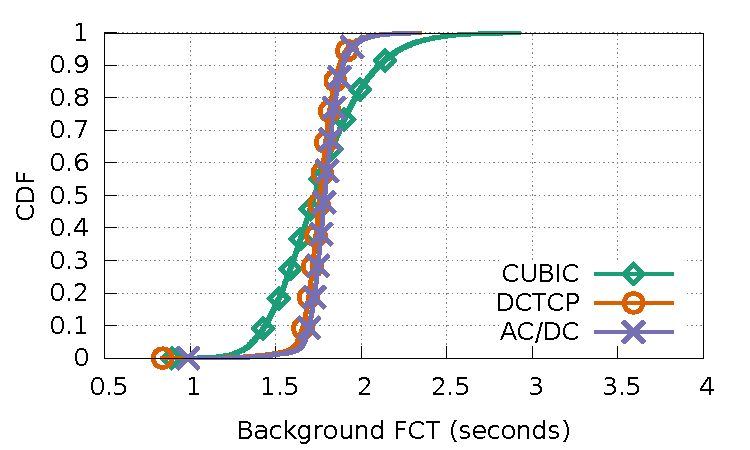
\includegraphics[width=\textwidth]{acdctcp/figures/macro_benchmarks/macro_4stride/stride4_big512MB_fct.pdf}
                \caption{Background flow completion times.}
                \label{macro_4stride_background_fct}
        \end{subfigure}
        \caption{CDF of mice and background FCTs in concurrent stride workload.}
        \label{macro_4stride_fct}
\end{figure*}

\begin{figure*}[!t]
        \centering
        \begin{subfigure}[b]{0.45\textwidth}
                \centering
                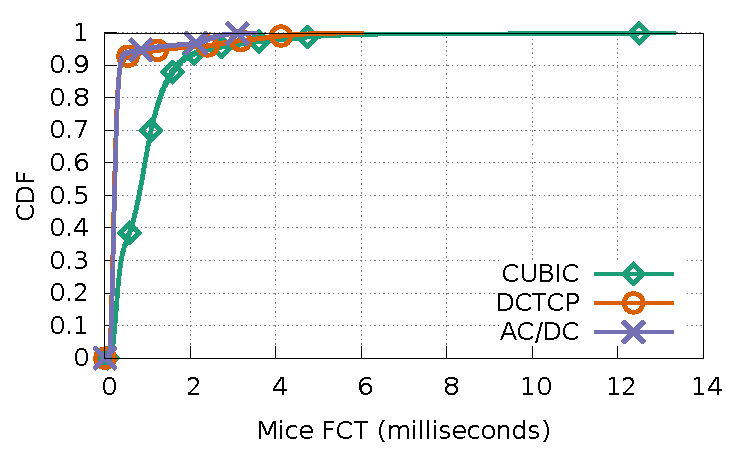
\includegraphics[width=\textwidth]{acdctcp/figures/macro_benchmarks/shuffle_17hosts/shuffle_mice16KB_fct.pdf}
                \caption{Mice flow completion times.}
                \label{macro_shuffle_mice_fct}
        \end{subfigure}
        \begin{subfigure}[b]{0.45\textwidth}
                \centering
                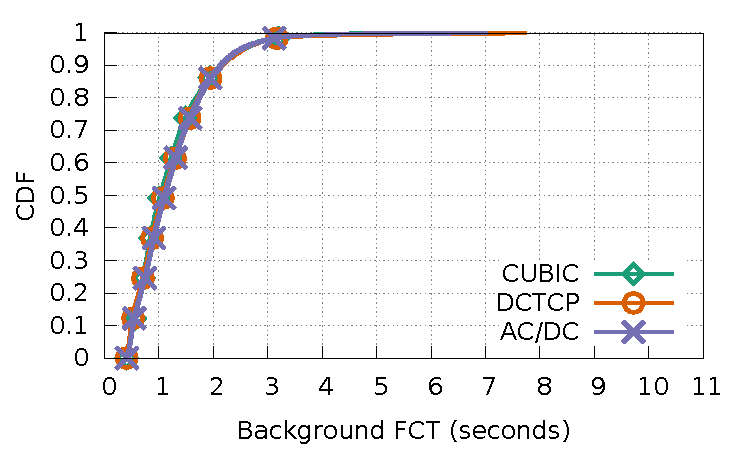
\includegraphics[width=\textwidth]{acdctcp/figures/macro_benchmarks/shuffle_17hosts/shuffle_big512MB_fct.pdf}
                \caption{Background flow completion times.}
                \label{macro_shuffle_background_fct}
        \end{subfigure}
        \caption{CDF of mice and background FCTs in shuffle workload.}
        \label{macro_shuffle_fct}
\end{figure*}

\begin{figure*}[!t]
        \centering
        \begin{subfigure}[b]{0.45\textwidth}
                \centering
                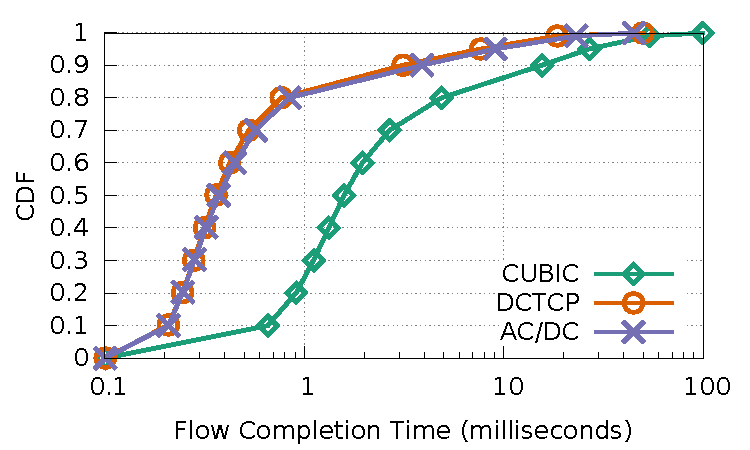
\includegraphics[width=\textwidth]{acdctcp/figures/macro_benchmarks/trace-driven/trace_driven_workload_dctcp_senders5_10points.pdf}
                \caption{Web-search workload.}
                \label{trace-driven-searching-fct}
        \end{subfigure}
        \begin{subfigure}[b]{0.45\textwidth}
                \centering
                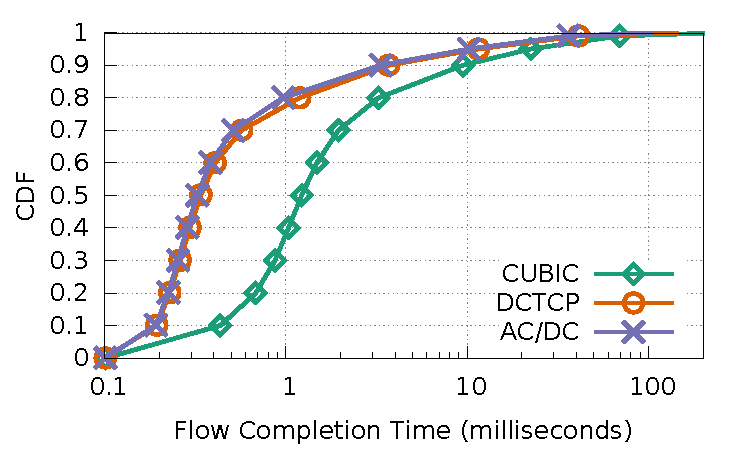
\includegraphics[width=\textwidth]{acdctcp/figures/macro_benchmarks/trace-driven/trace_driven_workload_conga_senders5_10points.pdf}
                \caption{Data-mining workload.}
                \label{trace-driven-data-mining-fct}
        \end{subfigure}
        \caption{CDF of mice ($<$10KB) FCT in web-search and data-mining workloads.}
        \label{macro-trace-driven-fct}
\end{figure*}
\fi


In this section we attach all servers to a single switch and
run a variety of workloads to better understand
how well~\acdc{} tracks DCTCP's performance. Experiments are run for 10 minutes. A simple TCP application
sends messages of specified sizes to measure FCTs.

\tightparagraph{Incast}
In this section, we evaluate incast scenarios.
To scale the experiment, 17 physical servers are equipped with four NICs each
and one flow is allocated per NIC.
In this way, incast can support up to 47-to-1 fan-in (our switch only has 48 ports).
We measure the extent of incast by increasing the number of concurrent senders to 16, 32, 40 and 47.
Figure~\ref{incast_9k_tput_fairness} shows throughput and fairness results.
Both DCTCP and \acdc{} obtain a fairness index greater than 0.99 and get comparable throughput as CUBIC.
Figure~\ref{incast_9k_sockperf_droprate} shows the RTT and packet drop rate results.
When there are 47 concurrent senders, DCTCP can reduce median RTT by 82\% and \acdc{} can reduce by 97\%;
DCTCP can reduce 99.9$^{th}$ percentile RTT by 94\% and \acdc{} can reduce by 98\%.
Both DCTCP and \acdc{} have 0\% packet drop rate. It is curious that~\acdc{}’s
performance is better than DCTCP when the number of senders increases (Figure~\ref{incast_9k_50th_sockperf}).
The Linux DCTCP code puts a lower bound of 2 packets on \cwnd{}.
In incast, we have up to 47 concurrent competing flows and
the network's MTU size is 9KB. In this case, the lower bound is too high,
so DCTCP's RTT increases gradually with the number of senders.
This issue was also found in~\cite{judd2015nsdi}.~\acdc{} controls \rwnd{} (which is in bytes)
instead of \cwnd{} (which is in packets) and \rwnd{}'s lowest value can be much smaller than 2*MSS.
We verified modifying~\acdc{}'s lower bound caused identical behavior.

\crs{The second test aims to put pressure on the switch's dynamic
buffer allocation scheme, similar to an experiment in the DCTCP paper~\cite{alizadeh2011data}.}
To this end, we aim to congest every switch port.
The 48 NICs are split into 2 groups: group $A$ and $B$.
Group $A$ has 46 NICs and $B$ has 2 (denoted $B_1$ and $B_2$).
Each of the 46 NICs in $A$ sends and receives 4 concurrent flows within $A$
(\ie{}, NIC $i$ sends to [$i+1$, $i+4$] mod 46).
Meanwhile, all of the NICs in $A$ send to $B_1$, creating a 46-to-1 incast.
This workload congests 47 out of 48 switch ports.
We measure the RTT between $B_2$ and $B_1$ (i.e., RTT of the traffic traversing the most congested port) and
the results are shown in Figure~\ref{sockperf_pressure_incast}.
The average throughputs for CUBIC, DCTCP, and~\acdc{} are 214, 214 and 201 Mbps respectively,
all with a fairness index greater than 0.98.
CUBIC has an average drop rate of 0.34\% but the most congested port has a drop rate as high as 4\%.
This is why the 99.9$^{th}$ percentile RTT for CUBIC is very high.
The packet drop rate for both DCTCP and~\acdc{} is 0\%.

\begin{figure*}[!t]
        \centering
        \begin{subfigure}[b]{0.45\textwidth}
                \centering
                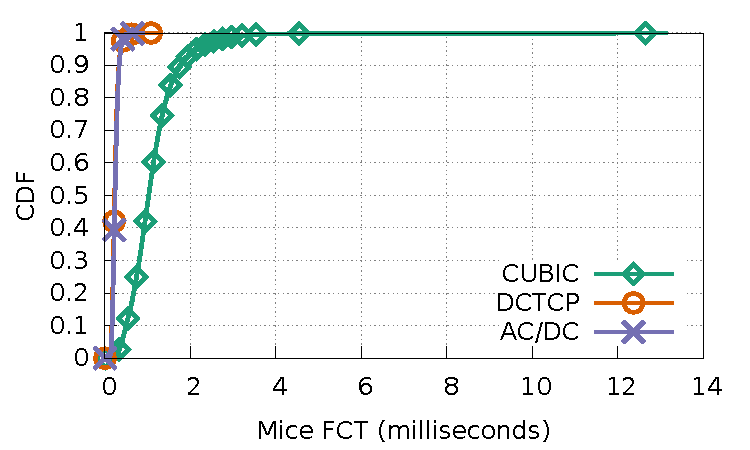
\includegraphics[width=\textwidth]{acdctcp/figures/macro_benchmarks/macro_4stride/stride4_mice16KB_fct.pdf}
                \caption{Mice flow completion times.}
                \label{macro_4stride_mice_fct}
        \end{subfigure}
        \begin{subfigure}[b]{0.45\textwidth}
                \centering
                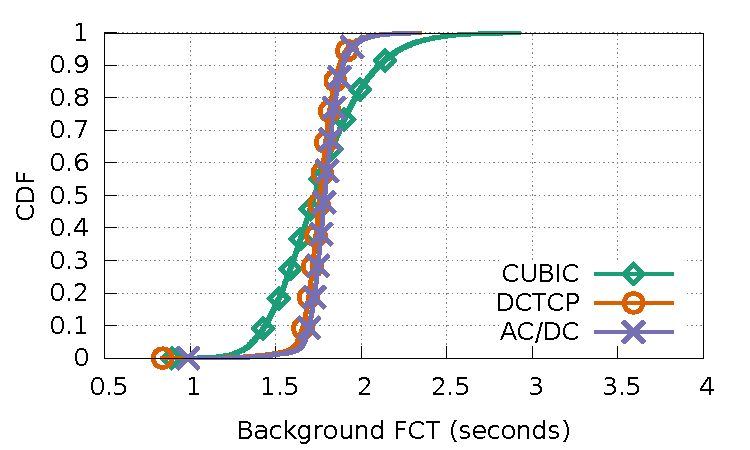
\includegraphics[width=\textwidth]{acdctcp/figures/macro_benchmarks/macro_4stride/stride4_big512MB_fct.pdf}
                \caption{Background flow completion times.}
                \label{macro_4stride_background_fct}
        \end{subfigure}
        \caption{CDF of mice and background FCTs in concurrent stride workload.}
        \label{macro_4stride_fct}
\end{figure*}

\begin{figure*}[!t]
        \centering
        \begin{subfigure}[b]{0.45\textwidth}
                \centering
                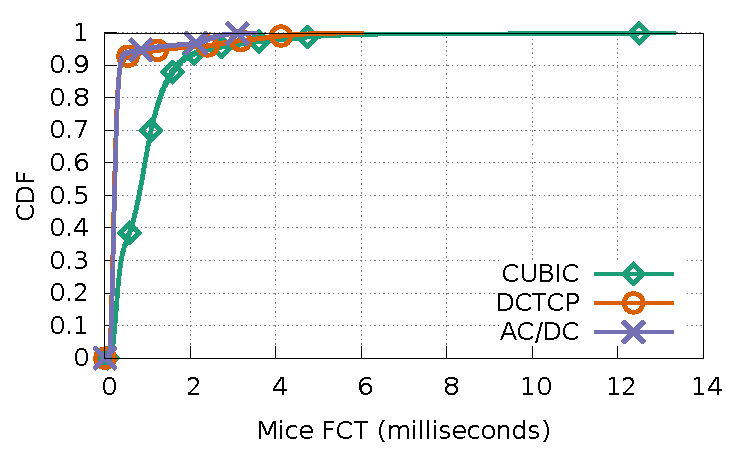
\includegraphics[width=\textwidth]{acdctcp/figures/macro_benchmarks/shuffle_17hosts/shuffle_mice16KB_fct.pdf}
                \caption{Mice flow completion times.}
                \label{macro_shuffle_mice_fct}
        \end{subfigure}
        \begin{subfigure}[b]{0.45\textwidth}
                \centering
                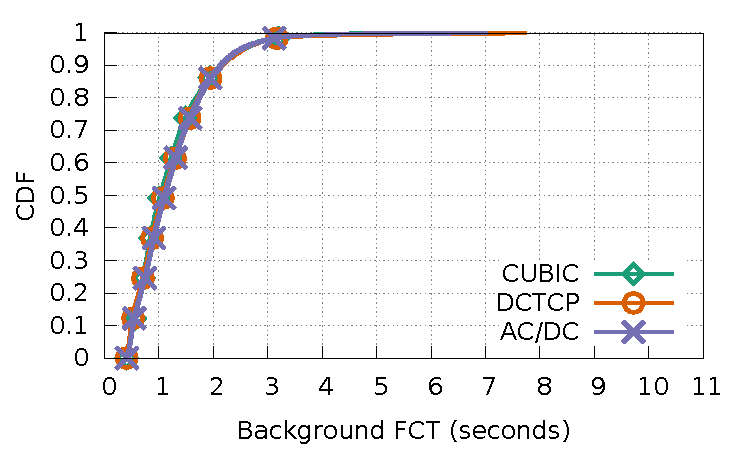
\includegraphics[width=\textwidth]{acdctcp/figures/macro_benchmarks/shuffle_17hosts/shuffle_big512MB_fct.pdf}
                \caption{Background flow completion times.}
                \label{macro_shuffle_background_fct}
        \end{subfigure}
        \caption{CDF of mice and background FCTs in shuffle workload.}
        \label{macro_shuffle_fct}
\end{figure*}

\begin{figure*}[!t]
        \centering
        \begin{subfigure}[b]{0.45\textwidth}
                \centering
                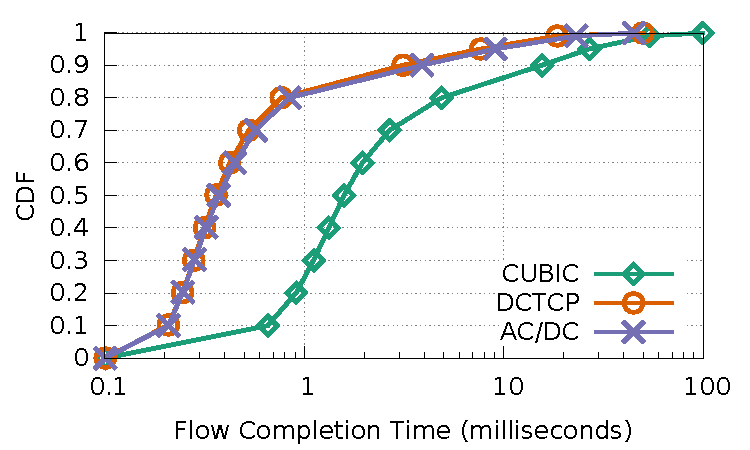
\includegraphics[width=\textwidth]{acdctcp/figures/macro_benchmarks/trace-driven/trace_driven_workload_dctcp_senders5_10points.pdf}
                \caption{Web-search workload.}
                \label{trace-driven-searching-fct}
        \end{subfigure}
        \begin{subfigure}[b]{0.45\textwidth}
                \centering
                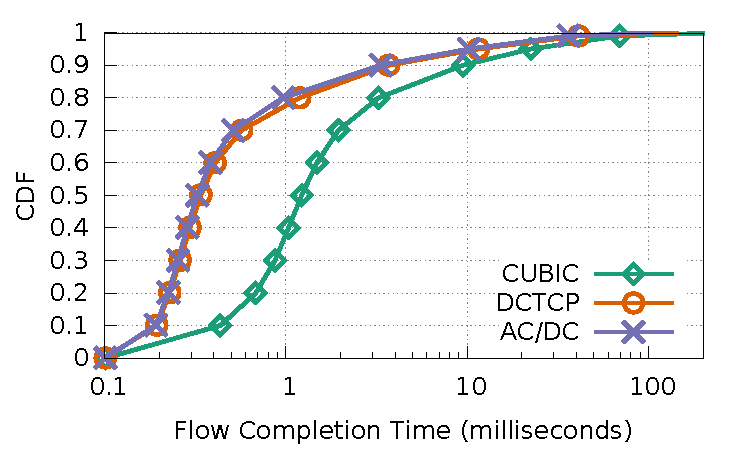
\includegraphics[width=\textwidth]{acdctcp/figures/macro_benchmarks/trace-driven/trace_driven_workload_conga_senders5_10points.pdf}
                \caption{Data-mining workload.}
                \label{trace-driven-data-mining-fct}
        \end{subfigure}
        \caption{CDF of mice (flows$<$10KB) FCT in web-search and data-mining workloads.}
        \label{macro-trace-driven-fct}
\end{figure*}

\tightparagraph{Concurrent stride workload}
In concurrent stride, 17 servers are attached to a single switch.
Each server $i$ sends a 512MB flow to servers [$i+1$, $i+4$] mod 17 in sequential fashion
to emulate background traffic.
Simultaneously, each server $i$ sends 16KB messages every 100 ms to 
server $(i+8)$ mod 17.
The FCT for small flows (16KB) and background flows (512MB) are shown 
in Figure~\ref{macro_4stride_fct}. For small flows, DCTCP and \acdc{} 
reduce the median FCT by 77\% and 76\% respectively. 
At the 99.9$^{th}$ percentile, DCTCP and \acdc{} reduce FCT by 91\% and 93\%, respectively.
For background flows, DCTCP and \acdc{} offer similar completion times.
CUBIC has longer background FCT because its fairness is not as 
good as DCTCP and \acdc{}.


\tightparagraph{Shuffle workload}
In shuffle, each server sends 512MB to every other server in random order. 
A sender sends at most 2 flows simultaneously and when
a transfer is finished, the next one is started until 
all transfers complete.
Every server $i$ also sends a 16 KB message to server $(i+8)$ mod 17 
every 100 ms. This workload is repeated for 30 runs.
The FCT for each type of flow is shown in Figure~\ref{macro_shuffle_fct}.
For small flows, DCTCP and \acdc{} reduce median FCT by
72\% and 71\% when compared to CUBIC. 
At the 99.9$^{th}$ percentile, DCTCP and \acdc{} 
reduce FCTs by 55\% and 73\% respectively.
For large flows, CUBIC, DCTCP and \acdc{} have almost identical performance.


\tightparagraph{Trace-driven workloads}
Finally, we run trace-driven workloads. 
An application on each server builds a long-lived TCP connection with every other server.
Message sizes are sampled from a trace and sent to a random destination in sequential fashion. Five
concurrent applications on each server are run to increase network load. Message
sizes are sampled from a web-search~\cite{alizadeh2011data}
and a data-mining workload~\cite{greenberg2009vl2,alizadeh2014conga}, whose flow size distribution has a heavier tail.
Figure~\ref{macro-trace-driven-fct} shows a CDF of FCTs for mice flows (smaller than 10KB) 
in the web-search and data-mining workloads.
In the web-search workload,
DCTCP and \acdc{} reduce median FCTs by 77\% and 76\%, respectively. 
At the 99.9$^{th}$ percentile, DCTCP and \acdc{} reduce FCTs by 50\% and 55\%, respectively.
In the data-mining workload, DCTCP and \acdc{} reduce median FCTs by 72\% and 73\%, respectively. 
At the 99.9$^{th}$ percentile, DCTCP and \acdc{} reduce FCTs by 36\% and 53\% respectively.  
%In both workloads, DCTCP and \acdc{} improve the fraction of mice flows that finish 
%in 1 millisecond significantly (from 20\%/30\% to 80\%).

\tightparagraph{Evaluation summary}
The results validate that congestion control can be accurately implemented in the vSwitch.
~\acdc{} tracks the performance of an unmodified host DCTCP stack
over a variety of workloads with little computational overhead.
Furthermore,~\acdc{} provides this functionality over 
various host TCP congestion control configurations. 

